%\documentclass{article}
\documentclass[10pt,a4paper]{article}
\usepackage[top=30pt,bottom=30pt,left=48pt,right=46pt]{geometry}

\usepackage[utf8]{inputenc}

\title{Book of Solutions}
\author{C Thierfelder}
\date{May 2020}

\usepackage{natbib}

%MATH
\usepackage{amsmath}
\usepackage{amsfonts}

%PAGELAYOUT
\usepackage{a4wide}

%GRAPHICS
\usepackage{graphicx}
\usepackage[dvipsnames]{xcolor}
\usepackage{tikz}
\usetikzlibrary{shapes}
\usetikzlibrary{plotmarks}

%HYPERLINKS
\usepackage{hyperref}
\hypersetup{
    colorlinks=true,
    linkcolor=blue,
    filecolor=magenta,      
    urlcolor=cyan,
}

\usepackage[shortlabels]{enumitem}

\begin{document}

\maketitle

\section{Introduction}
There is a theory which states that if ever anyone discovers exactly what the Universe is for and why it is here, it will instantly disappear and be replaced by something even more bizarre and inexplicable.
There is another theory which states that this has already happened.

\begin{figure}[h!]
\centering
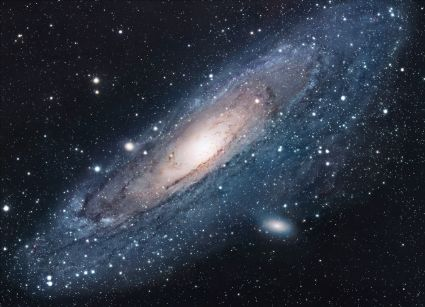
\includegraphics[scale=1.7]{universe}
\caption{The Universe}
\label{fig:universe}
\end{figure}

\newpage
\tableofcontents

%SECTION_NUMBERING
\setcounter{secnumdepth}{2}

\newpage
\section{Primer special relativity}
Definition of line element
\begin{align}
    ds^2 &= dx^\mu dx_\nu = \eta_{\mu\nu}dx^\mu dx^\nu\\
        &= dx^T\eta dx
\end{align}
Definition of Lorentz transformation
\begin{align}
    dx^\mu = \Lambda^\mu_{\;\nu}dx^\nu
\end{align}
By postulate the line element $ds$ is invariant under Lorentz transformation
\begin{align}
    ds^2 &= \eta_{\mu\nu}dx^\mu dx^\nu\\
    &\stackrel{!}{=} \eta_{\alpha\beta}\Lambda^\alpha_{\;\mu}dx^\mu \Lambda^\beta_{\;\nu}dx^\nu\quad\rightarrow\quad \eta_{\mu\nu} = \eta_{\alpha\beta}\Lambda^\alpha_{\;\mu} \Lambda^\beta_{\;\nu}
\end{align}
or analog
\begin{align}
    ds^2 &= dx^T\eta dx\\
    &\stackrel{!}{=} (\Lambda dx)^T\eta (\Lambda dx)\\
    &= dx^T\Lambda^T\eta \Lambda dx\quad\rightarrow\quad \eta = \Lambda^T\eta\Lambda
\end{align}
Observation with the eigentime $d\tau=ds/c$ and 3-velocity $dx^i = v^i dt$
\begin{align}
    \frac{ds^2}{d\tau^2}=c^2&=c^2\frac{dt^2}{d\tau^2}-\frac{dx^i}{dt}\frac{dx_i}{dt}\left(\frac{dt}{d\tau}\right)^2\\
    1&=\frac{dt^2}{d\tau^2}\left(1-\frac{v^iv_i}{c^2}\right)\quad\rightarrow\quad\frac{dt}{d\tau}\equiv\gamma=\left(\sqrt{1-\frac{v^2}{c^2}}\right)^{-1}
\end{align}
Definition of 4-velocity with 3-velocity $d\vec{x} = \vec{v} dt$
\begin{align}
    u^\mu\equiv\frac{dx^\mu}{d\tau}&=\frac{dx^\mu}{dt}\frac{dt}{d\tau}=\quad\rightarrow\quad u^\mu u_\mu=\eta_{\mu\nu}\frac{dx^\mu}{d\tau} \frac{dx^\nu}{d\tau}=\frac{ds^2}{d\tau^2}=c^2\\
    &=(c,\vec{v})\gamma
\end{align}
Object moving in $x$ direction with $v$ meaning $dx=v\cdot dt$ compared to
rest frame $dx'=0$
\begin{align}
    c^2dt'^2=ds^2 &= c^2dt^2- v^2 dt^2\\
    &=c^2dt^2\left(1-\frac{v^2}{c^2}\right)\\
    dt'=\frac{ds}{c}\equiv d\tau&=dt\sqrt{1-\frac{v^2}{c^2}}=\frac{dt}{\gamma}
\end{align}
Definition 4-momentum (using the 3-momentum $\vec{p}=\gamma m\vec{v}$)
\begin{align}
    p^\mu \equiv mu^\mu=(\gamma mc,\gamma m\vec{v})=\left(\frac{E_p}{c},\vec{p}\right)\quad&\rightarrow\quad p^\mu p _\mu=m^2u^\mu u_\mu=m^2c^2\\
    &\rightarrow\quad (p^0)^2-p^ip_i=m^2c^2\\
    &\rightarrow\quad p^0=\sqrt{m^2c^2+\vec{p}^2}\\
    &\rightarrow\quad E_p=\sqrt{m^2c^4+\vec{p}^2c^2}\\
    &\qquad\qquad=\frac{mc^2}{\sqrt{1-\frac{\vec{v}^2}{c^2}}}
\end{align}

\section{Groups}
\subsection{SO(3)}

\subsection{SU(2)}
Finite dimensional irreps of the Lorentz group are labeled by $l$ with
\begin{align}
    l &\in \left\{0,\frac{1}{2},1,\frac{3}{2},2,...\right\}.
\end{align}
and have dimension $2l+1$. For two irreps with $l\ge m$ the tensor product representations decomposes as
\begin{align}
    V_l \otimes V_m &\cong V_{l+m}\oplus V_{l+m-1}\oplus ... \oplus V_{l-m+1}\oplus V_{l-m}\\
    \text{dim}(V_l \otimes V_m)&=(2l+1)(2m+1)\\
    \text{dim}(V_{l+m} \oplus ...\oplus V_{l-m})&=\sum_{k=0}^{2m}2[(l-m)+k]+1\\
    &=(2m+1)[2(l-m)+1]+2\frac{2m(2m+1)}{2}\\
    &=(2m+1)(2l+1)
\end{align}

\subsection{SU(3)}

\subsection{Lorentz group O(1,3)}
Finite dimensional irreps of the Lorentz group are labeled by two parameters $(\mu,\nu)$ with
\begin{align}
    \mu,\nu &\in \left\{0,\frac{1}{2},1,\frac{3}{2},2,...\right\}.
\end{align}
and have dimension $(2\mu+1)(2\nu+1)$
\begin{align*}
    M^2&=\mu(\mu+1)\\
    N^2&=\nu(\nu+1)\\
    j  &\in |\mu-\nu|, ..., (\mu+\nu)
\end{align*}


\begin{center}
 \begin{tabular}{c c c l} 
 \hline
 irrep & dim & j & example \\ [0.5ex] 
 \hline\hline
 $(0,0)$                        & 1 & 0 & Scalar \\  [0.5ex]
 $(\frac{1}{2},0)$              & 2 & $\frac{1}{2}$ & Left-handed Weyl spinor \\  [0.5ex]
 $(0,\frac{1}{2})$              & 2 & $\frac{1}{2}$ & Right-handed Weyl spinor \\  [0.5ex]
 $(\frac{1}{2},\frac{1}{2})$    & 4 & 0,1 & 4-Vector $A^\mu$ \\  [0.5ex]
 $(1,0)$                        & 3 & 1 & Self-dual 2-form \\  [0.5ex]
 $(0,1)$                        & 3 & 1 & Anti-self-dual 2-form \\  [0.5ex]
 $(1,1)$                        & 9 & 0,1,2 & Traceless symmetric $2^\text{nd}$ rank tensor \\ \hline  \\ [0.5ex]
  \hline
 rep & dim & j & example \\ [0.5ex] 
 \hline\hline
 $(\frac{1}{2},0)\oplus(0,\frac{1}{2})$& - & - & Dirac bispinor $\psi^\alpha\quad \alpha\in\{1,2,3,4\}$ \\  [0.5ex]
 $(\frac{1}{2},\frac{1}{2})\otimes\left[(\frac{1}{2},0)\oplus(0,\frac{1}{2})\right]$& - & - & Rarita-Schwinger field $\psi^\alpha\quad \alpha\in\{1,2,3,4\}$ \\  [0.5ex]
  $(0,1)\oplus(0,1)$& - & - & Parity invariant field of 2-forms\\ \hline \\ [0.5ex]
\end{tabular}
\end{center}



\newpage
\section{Useful formulas}
Starting from the Fourier integral theorem we have some freedom to distribute the $2\pi$ between back and forth transformation ($a,b\in\mathbb{R}$)
\begin{align}
    F(k)=\sqrt{\frac{|b|}{(2\pi)^{1-a}}}\int_{-\infty}^\infty f(x)e^{ibkx}dx\quad\leftrightarrow\quad f(x)=\sqrt{\frac{|b|}{(2\pi)^{1+a}}}\int_{-\infty}^\infty F(t)e^{-ibkx}dk
\end{align}

\begin{align}
    \int\delta(x)e^{-ikx}dx&=1\\
    \int e^{ik(x-y)}dk&=2\pi\delta(x-y)
\end{align}


\newpage

\section{Mathematical}
\subsection{{\sc Woit} - Quantum Theory, Groups and Representations}
\subsubsection{Problem B.1-4}
The time evolution is given by
\begin{align}
    |\Psi(t)\rangle&=e^{-iHt}|\Psi(0)\rangle\\
    &=\left(\sum_{k=0}^\infty\frac{(-iHt)^k}{k!}\right)|\Psi(0)\rangle
\end{align}
We see
\begin{align}
H=\left(
\begin{array}{ccc}
 0 & 1 & 0 \\
 1 & 0 & 0 \\
 0 & 0 & 2 \\
\end{array}
\right)\qquad
H^2=\left(
\begin{array}{ccc}
 1 & 0 & 0 \\
 0 & 1 & 0 \\
 0 & 0 & 4 \\
\end{array}
\right)
\qquad
H^3=\left(
\begin{array}{ccc}
 0 & 1 & 0 \\
 1 & 0 & 0 \\
 0 & 0 & 8 \\
\end{array}
\right)
\end{align}
and calculate
\begin{align}
    =\sum_{k=0}^\infty\frac{(-it)^{2k}}{(2k)!}&=\sum_{k=0}^\infty(-1)^k \frac{t^{2k}}{(2k)!}=\cos(t)\\
    \sum_{k=0}^\infty\frac{(-it)^{2k+1}}{(2k+1)!}&=(-i)\sum_{k=0}^\infty(-1)^{k}\frac{t^{2k+1}}{(2k+1)!}=-i\sin(t)\\
    \sum_{k=0}^\infty\frac{(-i2t)^k}{k!}&=\cos(2t)-i\sin(2t)=e^{-i2t}
\end{align}
which gives
\begin{align}
    e^{-iHt}=\left(
\begin{array}{ccc}
 \cos (t) & -i \sin (t) & 0 \\
 -i \sin (t) & \cos (t) & 0 \\
 0 & 0 & e^{-2 i t} \\
\end{array}
\right)
\end{align}
and therefore
\begin{align}
|\Psi(t)\rangle=\left(
\begin{array}{ccc}
 \psi_1\cos (t)  -\psi_2i \sin (t) \\
 -\psi_1i \sin (t) + \psi_2\cos (t) \\
 \psi_3e^{-2 i t} \\
\end{array}
\right)
\end{align}.
To check the result one can calculate both sides of $i\partial_t|\Psi(t)\rangle=H|\Psi(t)\rangle$.

\subsection{{\sc Baez, Muniain} - Gauge Fields, Knots and Gravity}
\subsubsection{Problem I.1 - Plane waves in vacuum}
With
\begin{align}
    \vec{\mathcal{E}}=\vec{E}e^{-i(\omega t -\vec{k}\vec{x})}
\end{align}
we calculate in cartesian coordinates 
\begin{enumerate}
    \item $\nabla\cdot\vec{\mathcal{E}}=0$
\begin{align}
    \nabla\cdot\vec{\mathcal{E}}&=\partial_a\mathcal{E}_a\\
    &=\partial_a(e^{-i(\omega t -\vec{k}\vec{x})})E_a\vec{e}^a\\
    &=\delta_{ab}ik_bE_a e^{-i(\omega t -\vec{k}\vec{x})}\vec{e}^a\\
    &=ik_bE_b e^{-i(\omega t -\vec{k}\vec{x})}\vec{e}^a\\
    &=0
\end{align}
where we assumed $E_a=\text{const}$ and used
\begin{align}
    0&=\vec{k}\cdot\vec{E}\\
    &=k_a\vec{e}^aE_a\vec{e}^a\\
    &=k_aE_a
\end{align}

\item $\nabla\times\vec{\mathcal{E}}=i\frac{\partial\vec{\mathcal{E}}}{\partial t}$
\begin{align}
    \nabla\times\vec{\mathcal{E}}&=\epsilon_{abc}\partial_b\mathcal{E}_c\vec{e}_a \\
    &=\epsilon_{abc}E_c\vec{e}_a\partial_b(e^{-i(\omega t -\vec{k}\vec{x})}) \\
    &=\epsilon_{abc}E_c\vec{e}_a\delta_{bd}ik_de^{-i(\omega t -\vec{k}\vec{x})} \\
    &=i(\epsilon_{abc}k_bE_c\vec{e}_a)e^{-i(\omega t -\vec{k}\vec{x})} \\
    &=i(-i\omega E_a\vec{e}^a)e^{-i(\omega t -\vec{k}\vec{x})} \\
    &=i(E_a\vec{e}^a)(-i\omega) e^{-i(\omega t -\vec{k}\vec{x})} \\
    &=i\vec{E}\frac{\partial}{\partial t} e^{-i(\omega t -\vec{k}\vec{x})} \\
    &=i\frac{\partial\vec{\mathcal{E}}}{\partial t}
\end{align}
where we used (typo in the book!)
\begin{align}
    -i\omega\vec{E}&=\vec{k}\times\vec{E}\\
    &=\epsilon_{abc}k_bE_c\vec{e}_a
\end{align}

\end{enumerate}

\section{Quantum Field Theory}
\subsection{{\sc Srednicki} - Quantum Field Theory}
\subsubsection{Problem 6.1 - Path integral in quantum mechanics}
\begin{align}
    \langle q'',t''|q',t'\rangle&=\int\mathcal{D}q\mathcal{D}p\exp\left[i\int_{t'}^{t''}dt\left(p(t)\dot{q}(t)-H(p(t),q(t))\right)\right]\\
    &=\int\prod_{j=0}^{N}dq_j\prod_{k=1}^N\frac{dp_k}{2\pi}e^{ip_k(q_{j+1}-q_j)}e^{-iH(p_k,\bar{q}_j)\delta t}\
\end{align}



\section{Quantum Gravity}
\subsection{{\sc Ammon, Erdmenger} - Gauge/Gravity Duality - Foundations and Applications}
The authors use $d-1$ spacial dimension and the sign convention 
\begin{align}
\eta_{\mu\nu}=diag(-1,1,...,1)
\end{align}
which implies 
\begin{align}
    \square&=\partial^\mu\partial_\mu=-\partial_t^2+\triangle\\
    kx&=-k^0x^0+\vec{k}\vec{x}
\end{align}
and results in a minus sign in the KG equation.

\subsubsection{Problem 1.1.1 - Fourier representation of free scalar field}
Ansatz (because KG equation looks quite similar to wave equation) $\phi(x)=a\cdot e^{ikx}$ with $x^\mu=(t,\vec{x})$, $k^\mu=(\omega,\vec{k})$ and $a\in\mathbb{C}$ meaning 
\begin{align}
    e^{ikx}\equiv e^{ik^{\mu}x_{\mu}}=e^{i\eta_{\mu\nu}k^{\mu}x^{\nu}}=e^{i(-k^0x^0+\vec{k}\vec{x})}
\end{align}
Inserting into the equation of motion
\begin{align}
    (\square - m^2)\phi(x)&=(\partial^t\partial_t + \triangle - m^2)\phi(x)\\
    &=a(-\partial_t^2 + \triangle - m^2)e^{i(-\omega t+\vec{k}\vec{x})}\\
    &=a\left(\omega^2 + i^2\vec{k}^2 - m^2\right)e^{i(-\omega t+\vec{k}\vec{x})}=0 
\end{align}
This implies $\omega^2-\vec{k}^2-m^2=0$ and therefore $\omega_k\equiv\omega=\sqrt{\vec{k}^2+m^2}$. One particular solution is therefore $\phi(x)=a\cdot e^{ikx}|_{k^0=\omega_k}$. The general solution is then given by a superposition
\begin{align}
    \phi(x)=\int d^{d-1}\vec{k}\left[a(\vec{k})e^{ikx}\right]
\end{align}
to ensure a real valued $\phi{x}$ we add the conjugate complex solution
\begin{align}
    \phi(x)=\int d^{d-1}\vec{k}\left[a(\vec{k})e^{ikx} + a^*(\vec{k})e^{-ikx}\right].
\end{align}
The factor $(2\pi)^{1-d}/2\omega_k$ can be absorbed into $a(k)$.

\subsubsection{Problem 1.1.2 - Lagrangian of self-interacting scalar field}
The Lagrangian is then
\begin{align}
    \mathcal{L}&=\mathcal{L}_\text{free}+\mathcal{L}_\text{int}\\
                &=-\frac{1}{2}\eta^{\mu\nu}\partial_\mu\phi(x)\partial_\nu\phi(x)-\frac{1}{2}m^2\phi(x)^2-\frac{g}{4!}\phi(x)^4.
\end{align}
with the Euler-Lagrange equations
\begin{align}
    \partial_\alpha\left(\frac{\partial\mathcal{L}}{\partial(\partial_\alpha\phi)}\right)-\frac{\partial\mathcal{L}}{\partial\phi}=0.
\end{align}
Therefore
\begin{align}
    \partial_\alpha\left(\frac{\partial\mathcal{L}}{\partial(\partial_\alpha\phi)}\right)
    &=\partial_\alpha\left(-\frac{1}{2}\eta^{\mu\nu}[\delta_{\mu\alpha}\partial_\nu\phi+\partial_\mu\phi\delta_{\nu\alpha}]\right)\\
    &=\partial_\alpha\left(-\frac{1}{2}\eta^{\alpha\nu}\partial_\nu\phi-\frac{1}{2}\eta^{\mu\alpha}\partial_\mu\phi\right)\\
    &=-\partial_\alpha\left(\eta^{\alpha\beta}\partial_\beta\phi\right)\\
    &=-\partial^\beta\partial_\beta\phi\\
    &=-\square\phi
\end{align}
and
\begin{align}
    \frac{\partial\mathcal{L}}{\partial\phi} = -m^2\phi-\frac{g}{3!}\phi^3.
\end{align}

The relevant term in the Euler-Lagrange equations is $\partial\mathcal{L}_\text{int}/\partial\phi=-g\phi^3/3!$. The modified equation of motion is therefore
\begin{align}
    (\square - m^2)\phi(x)-\frac{g}{3!}\phi(x)^3=0
\end{align}

\subsubsection{Problem 1.1.3 - Complex scalar field }
\begin{align}
    \mathcal{L}_\text{free}&=-\partial_\mu\phi^*\partial^\mu\phi-m^2\phi^*\phi\\
    &=-\eta^{\mu\nu}\partial_\mu\phi^*\partial_\nu\phi-m^2\phi^*\phi\\
    &=-\frac{1}{2}\eta^{\mu\nu}\partial_\mu(\phi_1-i\phi_2)\partial_\nu(\phi_1+i\phi_2)-\frac{1}{2}m^2(\phi_1^2+\phi_2^2)\\
    &=-\frac{1}{2}\eta^{\mu\nu}\left(
    \partial_\mu\phi_1\partial_\nu\phi_1
    +i\partial_\mu\phi_1\partial_\nu\phi_2
    -i\partial_\mu\phi_2\partial_\nu\phi_1
    +\partial_\mu\phi_2\partial_\nu\phi_2
    \right)-\frac{1}{2}m^2(\phi_1^2+\phi_2^2)\\
    &=-\frac{1}{2}\eta^{\mu\nu}\left(\partial_\mu\phi_1\partial_\nu\phi_1+\partial_\mu\phi_2\partial_\nu\phi_2\right)-\frac{1}{2}m^2(\phi_1^2+\phi_2^2)\\
    &=-\frac{1}{2}\eta^{\mu\nu}\partial_\mu\phi_1\partial_\nu\phi_1-\frac{1}{2}m^2\phi_1^2
    -\frac{1}{2}\eta^{\mu\nu}\partial_\mu\phi_2\partial_\nu\phi_2-\frac{1}{2}m^2\phi_2^2\\
    &=\mathcal{L}_\text{free1}+\mathcal{L}_\text{free2}
\end{align}

Equations of motion for $\phi$ and $\phi^*$ are given by
\begin{align}
    \partial_\alpha\left(\frac{\partial\mathcal{L}}{\partial(\partial_\alpha\phi^*)}\right)-\frac{\partial\mathcal{L}}{\partial\phi^*}=0\\
    %
    -\partial_\mu\partial^\mu\phi+m^2\phi=0\\
    (\square-m^2)\phi=0
\end{align}
and
\begin{align}
    \partial_\alpha\left(\frac{\partial\mathcal{L}}{\partial(\partial_\alpha\phi^*)}\right)-\frac{\partial\mathcal{L}}{\partial\phi}=0\\
    %
    -\partial_\mu\partial^\mu\phi+m^2\phi^*=0\\
    (\square-m^2)\phi^*=0
\end{align}

\subsubsection{Problem 1.2.1 - Time-independence of Noether charge}
The conserved current is
\begin{align}
    \partial_\mu\mathcal{J}^\mu\equiv-\partial_0\mathcal{J}^0+\partial_i\mathcal{J}^i=0.
\end{align}
Spacial integration using Gauss law on the right hand side gives
\begin{align}
    \int_{\mathbb{R}^{d-1}} d^{d-1}\vec{x}\;\partial_0\mathcal{J}^0&=\int_{\mathbb{R}^{d-1}} d^{d-1}\vec{x}\;\partial_i\mathcal{J}^i\\
    %
    \partial_0\int_{\mathbb{R}^{d-1}} d^{d-1}\vec{x}\;\mathcal{J}^0&=\int_{\partial\mathbb{R}^{d-1}} dS\;\mathcal{J}^i\\
    \partial_0\mathcal{Q}&=0
\end{align}
where we used that $\mathcal{J}^i$ is vanishing at infinity.

\subsubsection{Problem 1.2.2 - Hamiltonian of scalar field}
The Lagrangian of the real free scalar field is given by 
\begin{align}
    \mathcal{L}=-\frac{1}{2}\eta^{\mu\nu}\partial_\mu\phi(x)\partial_\nu\phi(x)-\frac{1}{2}m^2\phi(x)^2.
\end{align}
The canonical momentum is therefore
\begin{align}
    \Pi &= \frac{\partial\mathcal{L}}{\partial(\partial_t\phi)}\\
    &=-\frac{1}{2}2\eta^{ti}\partial_i\phi -\frac{1}{2}2\eta^{tt}\partial_t\phi\\
    &=\partial_t\phi.
\end{align}
Using $\eta_{\mu\nu}=diag(-1,1,...,1)$ the Hamiltonian $\mathcal{H}=\Theta^{tt}=\eta^{t\nu}\Theta^t_{\;\nu}=-\Theta^t_{\;t}$ is 
\begin{align}
    \Theta^t_{\;t}
    &=-\frac{\partial\mathcal{L}}{\partial(\partial_t\phi)}\partial_t\phi+\mathcal{L}\\
    &=-\Pi\cdot\partial_t\phi+\mathcal{L}
\end{align}
and therefore
\begin{align}
    \mathcal{H}&=\Pi\partial_t\phi-\mathcal{L}\\
    &=\Pi^2-\left(-\frac{1}{2}\eta^{\mu\nu}\partial_\mu\phi(x)\partial_\nu\phi(x)-\frac{1}{2}m^2\phi(x)^2\right)\\
    &=\Pi^2-\left(\frac{1}{2}(\partial_t\phi)^2-\frac{1}{2}(\nabla\phi)^2-\frac{1}{2}m^2\phi(x)^2\right)\\
    &=\frac{1}{2}\Pi^2+\frac{1}{2}(\nabla\phi)^2+\frac{1}{2}m^2\phi(x)^2
\end{align}

\subsubsection{Problem 1.2.3 - Symmetric energy-momentum tensor}
The Lorentz transformation
\begin{align}
    \Lambda^\mu_{\;\nu}=\delta^\mu_{\;\nu}+\omega^\mu_{\;\nu}
\end{align}
implies the field transformation
\begin{align}
    \phi(x^\mu)\rightarrow\tilde\phi(x^\mu)&=\phi(x^\mu-\omega^\mu_{\;\rho}x^\rho)\\
    &=\phi(x^\mu)-\omega^\mu_{\;\rho}x^\rho\partial_\mu\phi
\end{align}
under which the Lagrangian transforms as
\begin{align}
    \mathcal{L}\rightarrow\tilde{\mathcal{L}}&=\mathcal{L}+\frac{\partial\mathcal{L}}{\partial x^\mu}dx^\mu\\
    &=\mathcal{L}-\omega^\nu_{\;\rho}x^\rho\partial_\mu(\delta^\mu_{\;\nu}\mathcal{L})\\
    &=\mathcal{L}+\partial_\mu(\omega^\nu_{\;\rho}x^\rho)\cdot(\delta^\mu_{\;\nu}\mathcal{L})-\partial_\mu(\omega^\nu_{\;\rho}x^\rho\delta^\mu_{\;\nu}\mathcal{L})\\
    &=\mathcal{L}+\omega^\nu_{\;\rho}\delta^\rho_\mu\cdot(\delta^\mu_{\;\nu}\mathcal{L})-\partial_\mu(\omega^\nu_{\;\rho}x^\rho\delta^\mu_{\;\nu}\mathcal{L})\\
    &=\mathcal{L}+\omega^\rho_{\;\rho}\mathcal{L}-\partial_\mu(\omega^\nu_{\;\rho}x^\rho\delta^\mu_{\;\nu}\mathcal{L})\\
    &=\mathcal{L}-\partial_\mu(\omega^\nu_{\;\rho}x^\rho\delta^\mu_{\;\nu}\mathcal{L})
\end{align}
where we used $\omega_{\mu\nu}=-\omega_{\nu\mu}$ meaning
\begin{align}
    \omega^\rho_{\;\rho}&=\eta^{\alpha\rho}\omega_{\alpha\rho}\\
    &=\sum_\rho\eta^{0\rho}\omega_{0\rho}+\eta^{1\rho}\omega_{1\rho}+\eta^{2\rho}\omega_{2\rho}+\eta^{3\rho}\omega_{3\rho}\\
    &=0
\end{align}    
in the last step (as $\eta$ has only diagonal elements and the diagonal elements of $\omega$ are zero). With $\delta\phi=-\omega^\mu_{\;\rho}x^\rho\partial_\mu\phi$ and $X^\mu=-\omega^\nu_{\;\rho}x^\rho\delta^\mu_{\;\nu}\mathcal{L}$ we obtain for the conserved current  
\begin{align}
    \mathcal{J}^\mu&=-\frac{\partial\mathcal{L}}{\partial(\partial_\mu\phi)}\delta\phi+X^\mu\\
    &=-\frac{\partial\mathcal{L}}{\partial(\partial_\mu\phi)}(-\omega^\nu_{\;\rho}x^\rho\partial_\nu\phi)+(-\omega^\nu_{\;\rho}x^\rho\delta^\mu_{\;\nu}\mathcal{L})\\
    &=(-\omega^\nu_{\;\rho}x^\rho)\left(-\frac{\partial\mathcal{L}}{\partial(\partial_\mu\phi)}\partial_\nu\phi+(\delta^\mu_{\;\nu}\mathcal{L})\right)\\
    &=(-\omega^\nu_{\;\rho}x^\rho)\Theta^\mu_{\;\nu}\\
    &=(-\eta^{\nu\alpha}\omega_{\alpha\rho}x^\rho)\Theta^\mu_{\;\nu}\\
    &=-\omega_{\alpha\rho}x^\rho\Theta^{\mu\alpha}\\
    &=-\frac{1}{2}\omega_{\alpha\rho}(x^\rho\Theta^{\mu\alpha}-x^\alpha\Theta^{\mu\rho})\\
    &=-\frac{1}{2}\omega_{\alpha\rho}N^{\mu\rho\alpha}
\end{align}
With $\partial_\mu\Theta^\mu_{\;\nu}=0$ and $\partial_\mu N^{\mu\nu\rho}=0$ we see
\begin{align}
    0&=\partial_\mu N^{\mu\nu\rho}\\
    &= \partial_\mu\left( x^\nu\Theta^{\mu\rho}-x^\rho\Theta^{\mu\nu}\right)\\
    &= (\partial_\mu x^\nu) \Theta^{\mu\rho}+  x^\nu (\partial_\mu \Theta^{\mu\rho}) -(\partial_\mu x^\rho)\Theta^{\mu\nu} - x^\rho (\partial_\mu\Theta^{\mu\nu})\\
    &= \delta_\mu^\nu \Theta^{\mu\rho}+  x^\nu (\partial_\mu \Theta^{\mu\rho}) -\delta_\mu^\rho\Theta^{\mu\nu} - x^\rho (\partial_\mu\Theta^{\mu\nu})\\
    &= \Theta^{\nu\rho} - \Theta^{\rho\nu}.
\end{align}
which means that the (canonical) energy-momentum tensor for Poincare invariant field theories is symmetric $\Theta^{\nu\rho} = \Theta^{\rho\nu}$.


\subsubsection{Problem 1.2.4 - Callan-Coleman-Jackiw energy-momentum tensor}
For the scalar field we have with $\mathcal{L}=-\frac{1}{2}\eta^{\alpha\beta}\partial_\alpha\phi\partial_\beta\phi-\frac{1}{2}m^2\phi^2$
\begin{align}
    \Theta^\mu_{\;\nu}&=-\frac{\partial\mathcal{L}}{\partial(\partial_\mu\phi)}\partial_\nu\phi+(\delta^\mu_{\;\nu}\mathcal{L})\\
    &=-\left(-\frac{1}{2}\eta^{\alpha\beta}\delta^\mu_{\alpha}\partial_\beta\phi-\frac{1}{2}\eta^{\alpha\beta}\partial_\alpha\phi\delta^\mu_{\beta}\right)\partial_\nu\phi +\delta^\mu_{\;\nu}\left(-\frac{1}{2}\eta^{\alpha\beta}\partial_\alpha\phi\partial_\beta\phi-\frac{1}{2}m^2\phi^2\right)\\
    &=\partial^\mu\phi\partial_\nu\phi -\frac{1}{2}\delta^\mu_{\;\nu}(\partial^\beta\phi\partial_\beta\phi+m^2\phi^2)
\end{align}
which gives in the massless case
\begin{align}
    \Theta^\mu_{\;\nu\text{, massless}}&=\partial^\mu\phi\partial_\nu\phi -\frac{1}{2}\delta^\mu_{\;\nu}\partial^\beta\phi\partial_\beta\phi\\
    \Theta_{\mu\nu\text{, massless}}&=\partial_\mu\phi\partial_\nu\phi -\frac{1}{2}\eta_{\mu\nu}\partial^\beta\phi\partial_\beta\phi
\end{align}

The new improved or Callan–Coleman–Jackiw energy-momentum tensor for a single, real, massless scalar field in $d$-dimensional Minkowski space is obtained by adding a term proportional to $(\partial_\mu\partial_\nu-\eta_{\mu\nu}\square)\phi^2$ where the proportionality constant is chosen to make the tensor traceless
\begin{align}
    T_{\mu\nu}=\partial_\mu\phi\partial_\nu\phi-\frac{1}{2}\eta_{\mu\nu}\partial_\rho\phi\partial^\rho\phi-\frac{d-2}{4(d-1)}\left(\partial_\mu\partial_\nu-\eta_{\mu\nu}\square\right)\phi^2
\end{align}
Let us now check the properties
\begin{enumerate}
    \item symmetric: obvious
    \item conserved: we use the equation of motion $\partial^\mu\partial_\mu\phi=\square\phi=0$
    \begin{align}
        \partial_\mu T^{\mu\nu}&=(\partial_\mu\partial^\mu\phi)\partial^\nu\phi+\partial^\mu\phi(\partial_\mu\partial^\nu\phi)\\
        &\quad-\frac{1}{2}\eta^{\mu\nu}\left[(\partial_\mu\partial_\rho\phi)\partial^\rho\phi + \partial_\rho\phi(\partial_\mu\partial^\rho\phi)\right]\\
        &\quad-\frac{d-2}{4(d-1)}\square\partial^\nu\phi^2+\frac{d-2}{4(d-1)}\eta^{\mu\nu}\partial_\mu\square\phi^2\\
        &=\partial^\mu\phi(\partial_\mu\partial^\nu\phi)-\frac{1}{2}\left[(\partial^\nu\partial_\rho\phi)\partial^\rho\phi + \partial_\rho\phi(\partial^\nu\partial^\rho\phi)\right]\\
        &=0
    \end{align}
    \item traceless: 
    \begin{align}
    T^\mu_{\;\mu}&=\partial^\mu\phi\partial_\mu\phi-\frac{1}{2}\eta^\mu_{\;\mu}\partial_\rho\phi\partial^\rho\phi-\frac{d-2}{4(d-1)}\left(\partial^\mu\partial_\mu-\eta^\mu_{\;\mu}\square\right)\phi^2\\
    &=\partial^\mu\phi\partial_\mu\phi-\frac{d}{2}\partial_\rho\phi\partial^\rho\phi-\frac{d-2}{4(d-1)}\left(\partial^\mu\partial_\mu-d\cdot\partial^\mu\partial_\mu\right)\phi^2\\
    &=\frac{2-d}{2}\partial_\rho\phi\partial^\rho\phi-\frac{d-2}{4(d-1)}(1-d)\partial^\mu\partial_\mu\phi^2\\
    &=\frac{2-d}{2}\partial_\rho\phi\partial^\rho\phi+\frac{d-2}{4}\partial^\mu\partial_\mu\phi^2\\
    &=\frac{2-d}{2}\partial_\rho\phi\partial^\rho\phi+\frac{d-2}{4}\partial^\mu(2\phi\partial_\mu\phi)\\
    &=\frac{2-d}{2}[\partial_\rho\phi\partial^\rho\phi-\partial^\mu\phi\partial_\mu\phi]+\frac{d-2}{2}\phi\cdot\square\phi\\
    &=0.
\end{align}
\end{enumerate}

\subsubsection*{Problem 1.2.5 - Noether currents of complex scalar field}
\begin{align}
    \mathcal{L}_\text{free}&=-\partial^\mu\phi^*\partial_\mu\phi-m^2\phi^*\phi\\
    &=-\eta^{\mu\nu}\partial_\nu\phi^*\partial_\nu\phi-m^2\phi^*\phi
\end{align}
with the field transformations
\begin{align}
    \phi\rightarrow\phi'&=e^{i\alpha}\phi=\phi+i\alpha\phi\\
    \phi^*\rightarrow\phi^{*'}&=e^{-i\alpha}\phi^*=\phi^*-i\alpha\phi^*\\
    \mathcal{L}\rightarrow\mathcal{L}'&=\mathcal{L}
\end{align}
we have $\delta\phi=i\alpha\phi$ and $\delta\phi^*=-i\alpha\phi^*$ and $X^\mu=0$. With 
\begin{align}
    \mathcal{J}^\sigma&=-\frac{\partial\mathcal{L}}{\partial(\partial_\sigma\phi)}\delta\phi+X^\sigma
\end{align}
we obtain the the two fields
\begin{align}    
    \mathcal{J}^\sigma&=-\frac{\partial\mathcal{L}}{\partial(\partial_\sigma\phi)}\delta\phi-\frac{\partial\mathcal{L}}{\partial(\partial_\sigma\phi^*)}\delta\phi^*\\
    &=-(\eta^{\sigma\nu}\partial_\nu\phi^*)i\alpha\phi+(\eta^{\sigma\nu}\partial_\nu\phi)i\alpha\phi^*\\
    &=i\alpha\left[\phi^*(\partial^\sigma\phi)-\phi(\partial^\sigma\phi^*)\right]
\end{align}

\subsubsection{Problem 1.2.6 - \texorpdfstring{$O(n)$}{Lg} invariance of action of \texorpdfstring{$n$}{Lg} free scalar fields}
For the $n$ real scalar fields with equal mass $m$ we have
\begin{align}
    \mathcal{L}=-\frac{1}{2}\sum_{j=1}^n\left[\eta^{\alpha\beta}(\partial_\alpha\phi_j)(\partial_\beta\phi^j)+m^2(\phi^j)^2\right]
\end{align}
the action functional is then
\begin{align}
    S&=\int d^dx\mathcal{L}\\
    &=-\frac{1}{2}\sum_{j=1}^n\int d^dx\left[\eta^{\alpha\beta}(\partial_\alpha\phi_j)(\partial_\beta\phi^j)+m^2(\phi_j\phi^j)\right]
\end{align}
With $\phi'^{j}=R^j_{\;k}\phi^k$ and the definition of an orthogonal matrix $R$ (inner product is invariant under rotation)
\begin{align}
    x^ix_i&=x^i\delta_{ij}x^j\\
    &\stackrel{!}{=}R^i_{\;a}x^a\delta_{ij}R^j_{\;b}x^b\\
    &=\delta_{ij}R^j_{\;b}R^i_{\;a}x^ax^b\\
    &=R_{ib}R^i_{\;a}x^ax^b
\end{align}
we require $R_{ib}R^i_{\;a}=\delta_{ba}$. Then we can recalculate the action
\begin{align}
    S'&=-\frac{1}{2}\sum_{j=1}^n\int d^dx\left[\eta^{\alpha\beta}(\partial_\alpha R_{ja}\phi^a)(\partial_\beta R^j_{\;b}\phi^b)+m^2(R_{ja}\phi^a\cdot R^j_{\;b}\phi^b)\right]\\
    &=-\frac{1}{2}\sum_{j=1}^n\int d^dx\left[\eta^{\alpha\beta}R_{ja}R^j_{\;b}(\partial_\alpha \phi^a)(\partial_\beta \phi^b)+m^2R_{ja}R^j_{\;b}(\phi^a\cdot \phi^b)\right]\\
    &=-\frac{1}{2}\sum_{b=1}^n\int d^dx\left[\eta^{\alpha\beta}\delta_{ab}(\partial_\alpha \phi^a)(\partial_\beta \phi^b)+m^2\delta_{ab}(\phi^a\cdot \phi^b)\right]\\
    &=-\frac{1}{2}\sum_{b=1}^n\int d^dx\left[\eta^{\alpha\beta}(\partial_\alpha \phi_b)(\partial_\beta \phi^b)+m^2(\phi_b\cdot \phi^b)\right]   
\end{align}
\textcolor{red}{Analog for the complex case.}

\subsubsection{Problem 1.3.1 - Field commutators of scalar field}
From the field  
\begin{align}
    \hat\phi(x)&=\frac{1}{(2\pi)^{d-1}}\int \frac{d^{d-1}\vec{k}}{2\omega_k}\left[\hat a(\vec{k})e^{ikx} + \hat a^\dagger(\vec{k})e^{-ikx}\right]_{k^0=\omega_k}
\end{align}
we can derive the conjugated momentum
\begin{align}
    \hat\Pi(x)&=\partial_t\hat\phi\\
    &=\frac{1}{(2\pi)^{d-1}}\int \frac{d^{d-1}\vec{k}}{2\omega_k}\partial_t\left[\hat a(\vec{k})e^{-i\omega_kt}e^{i\vec{k}\vec{x}} + \hat a^\dagger(\vec{k})e^{i\omega_kt}e^{-i\vec{k}\vec{x}}\right]\\
    &=\frac{1}{(2\pi)^{d-1}}\int \frac{d^{d-1}\vec{k}}{2\omega_k}\left[\hat a(\vec{k})(-i\omega_k)e^{ikx} + \hat a^\dagger(\vec{k})(i\omega_k)e^{-ikx}\right]_{k^0=\omega_k}\\
    &=\frac{i}{2(2\pi)^{d-1}}\int d^{d-1}\vec{k}\left[-\hat a(\vec{k})e^{ikx} + \hat a^\dagger(\vec{k})e^{-ikx}\right]_{k^0=\omega_k}.
\end{align}
Now calculating the three commutation relations
\begin{itemize}
\item $[\hat\phi(t,\vec{x}),\hat\phi(t,\vec{y})]$
\begin{align}
    &=\frac{1}{(2\pi)^{2(d-1)}}\int \frac{d^{d-1}\vec{k}d^{d-1}\vec{q}}{4\omega_k \omega_q}
    \left((\hat a(\vec{k})e^{ikx} + \hat a^\dagger(\vec{k})e^{-ikx})
    (\hat a(\vec{q})e^{iqy} + \hat a^\dagger(\vec{q})e^{-iqy})\right. - \\ 
    &\quad\left.(\hat a(\vec{q})e^{iqy} + \hat a^\dagger(\vec{q})e^{-iqy})
    (\hat a(\vec{k})e^{ikx} + \hat a^\dagger(\vec{k})e^{-ikx}) \right)
\end{align}
the bracket can then be simplified
\begin{align}
    (\hat a(\vec{k})&e^{ikx} + \hat a^\dagger(\vec{k})e^{-ikx})(\hat a(\vec{q})e^{iqy} + \hat a^\dagger(\vec{q})e^{-iqy})-(\hat a(\vec{q})e^{iqy} + \hat a^\dagger(\vec{q})e^{-iqy})
    (\hat a(\vec{k})e^{ikx} + \hat a^\dagger(\vec{k})e^{-ikx}) \\
    %
    &=[\hat a(\vec{k}),\hat a(\vec{q})]e^{i(kx+qy)}+[\hat a(\vec{k}),\hat a^\dagger(\vec{q})]e^{i(kx-qy)}+[\hat a^\dagger(\vec{k}),\hat a(\vec{q})]e^{i(-kx+qy)}+[\hat a^\dagger(\vec{k}),\hat a^\dagger(\vec{q})]e^{i(-kx-qy)}\\
    &=[\hat a(\vec{k}),\hat a^\dagger(\vec{q})]e^{i(kx-qy)}-[\hat a(\vec{q}),\hat a^\dagger(\vec{k})]e^{i(-kx+qy)}\\
    &=2\omega_k(2\pi)^{d-1}\left(\delta^{d-1}(\vec{k}-\vec{q})e^{i(kx-qy)}-\delta^{d-1}(\vec{q}-\vec{k})e^{i(-kx+qy)}\right)
\end{align}
where we used the given commutation relations for $\hat a(\vec{k})$.
\begin{align}
    [\hat\phi(t,\vec{x}),\hat\phi(t,\vec{y})] 
    &= \frac{1}{(2\pi)^{2(d-1)}}\int \frac{d^{d-1}\vec{k}d^{d-1}\vec{q}}{4\omega_k \omega_q}2\omega_k(2\pi)^{d-1}\left(\delta^{d-1}(\vec{k}-\vec{q})e^{i(kx-qy)}-\delta^{d-1}(\vec{q}-\vec{k})e^{i(-kx+qy)}\right)\\
    &= \frac{1}{(2\pi)^{d-1}}\int \frac{d^{d-1}\vec{k}d^{d-1}\vec{q}}{2 \omega_q}\left(\delta^{d-1}(\vec{k}-\vec{q})e^{i(kx-qy)}-\delta^{d-1}(\vec{q}-\vec{k})e^{i(-kx+qy)}\right)\\
    &= \frac{1}{(2\pi)^{d-1}}\int \frac{d^{d-1}\vec{k}d^{d-1}\vec{q}}{2 \omega_q}\left(\delta^{d-1}(\vec{k}-\vec{q})e^{i(-\omega_kt+\vec{k}\vec{x}-[-\omega_qt+\vec{q}\vec{y}]))}\right.\\
    &\qquad\qquad\qquad\qquad\left.-\delta^{d-1}(\vec{q}-\vec{k})e^{-i(-\omega_kt+\vec{k}\vec{x}-[-\omega_qt+\vec{q}\vec{y}]))}\right)\\
    &= \frac{1}{(2\pi)^{d-1}}\int \frac{d^{d-1}\vec{k}d^{d-1}\vec{q}}{2 \omega_q}\left(\delta^{d-1}(\vec{k}-\vec{q})e^{i(-[\omega_k-\omega_q]t+\vec{k}\vec{x}-\vec{q}\vec{y})}\right.\\
    &\qquad\qquad\qquad\qquad\left.-\delta^{d-1}(\vec{q}-\vec{k})e^{-i(-[\omega_k-\omega_q]t+\vec{k}\vec{x}-\vec{q}\vec{y})}\right)\\
    &= \frac{1}{(2\pi)^{d-1}}\int \frac{d^{d-1}\vec{k}}{2 \omega_k}\left(e^{i\vec{k}(\vec{x}-\vec{y})}-e^{-i\vec{k}(\vec{x}-\vec{y})}\right)\\
    &= \frac{1}{2 \omega_k}\left( \delta^{d-1}(\vec{y}-\vec{x})-\delta^{d-1}(\vec{x}-\vec{y})\right)\\
    &=0
\end{align}
where we used $\delta(x)=\int dk e^{-2\pi i kx}$ or $\delta^d(x)=\int \frac{d^dk}{(2\pi)^d} e^{-ikx}$.

\item $[\hat\Pi(t,\vec{x}),\hat\Pi(t,\vec{y})]$
\textcolor{red}{Not done yet}
\item $[\hat\phi(t,\vec{x}),\hat\Pi(t,\vec{y})]$
\textcolor{red}{Not done yet}
\end{itemize}

\subsubsection{Problem 1.3.2 - Lorentz invariant integration measure}
We use the property of the $\delta$-function $\delta(f(x))=\sum_i\frac{\delta(x-a_i)}{]f'(a_i)|}$ where ${a_i}$ are the zeros of $f(x)$ and $\omega_k=\sqrt{\vec{k}^2+m^2}$. With $\int d^dk$ being manifestly Lorentz invariant 
\begin{align}
    dk'^\mu = \Lambda^\mu_\nu dk^\nu\quad\rightarrow\quad \frac{dk'^\mu}{dk^\nu}=\Lambda^\mu_\nu\quad\rightarrow\quad\int d^d k'=|\text{det}(\Lambda^\mu_\nu)|\int d^dk=\int d^dk
\end{align}
$\delta^d[k^2+m^2]$ being invariant and with $k^0=\sqrt{\vec{k}^2+m^2}$ we see that $k$ is inside the forward light cone and remains there under orthochrone transformation ($\Theta(k^0)$ is invariant for relevant $k$) we are convinced that the starting expression is Lorentz invariant (integration over the upper mass shell)
\begin{align}
    \int d^{d}\vec{k} \delta^d[k^2+m^2]\Theta(k^0) &=\int d^{d-1}\vec{k}\int dk^0\delta^d[k^2+m^2]\Theta(k^0)\\
    &=\int d^{d-1}\vec{k}\int dk^0\delta^d[-(k^0)^2+\vec{k}^2+m^2]\Theta(k^0)\\
    &=\int d^{d-1}\vec{k}\int dk^0\delta^d[\omega_k^2-(k^0)^2]\Theta(k^0)\\
    &=\int d^{d-1}\vec{k}\int dk^0\left( \frac{\delta(k^0-\omega_k)}{2\omega_k}+\frac{\delta(k^0+\omega_k)}{2\omega_k} \right)\Theta(k^0)\\
    &=\int \frac{d^{d-1}\vec{k}}{2\omega_k}\int dk^0\delta(k^0-\omega_k)\\
    &=\int\frac{d^{d-1}\vec{k}}{2\omega_k}.
\end{align}
As we started with a Lorentz invariant expression the derived measure is also invariant.

\subsubsection{Problem 1.3.3 - Retarded Green function}
\begin{align}
    \Delta_\text{F}&=\int\frac{d^dk}{(2\pi)^d}\frac{e^{ik(x-y)}}{k^2+m^2-i\epsilon}\\
    G_\text{R}&=\int\frac{d^dk}{(2\pi)^d}\frac{e^{ik(x-y)}}{-(k^0+i\epsilon)^2+\vec{k}^2+m^2}
\end{align}
For the poles of $G_\text{R}$ we have
\begin{align}
    -(k^0+i&\epsilon)^2+\vec{k}^2+m^2 = 0\\
    k^0&=-i\epsilon\pm\sqrt{\vec{k}^2+m^2}\\
    &=-i\epsilon\pm\omega_k
\end{align}
while we the poles of $\Delta_\text{F}$ are given by
\begin{align}
    -(k^0)^2+&\vec{k^2}+m^2-i\epsilon=0\\
    k^0&=\pm\sqrt{\vec{k^2}+m^2-i\epsilon}\\
    &=\pm\sqrt{\omega_k^2-i\epsilon}
\end{align}
\begin{figure}[h]
\centering
\resizebox{5cm}{!}{%
    \begin{tikzpicture}
        \draw (-4,0) -- (4,0);
        \node[mark size=5pt,color=blue] at (+2,-0.5) {\pgfuseplotmark{triangle}};
        \node[mark size=5pt,color=blue] at (-2,+0.5) {\pgfuseplotmark{triangle}};
        \draw[red,thick] (-2,-0.5) circle (0.1cm);
        \draw[red,thick] (+2,-0.5) circle (0.1cm);
        \draw[black,thick] (-2,0) circle (0.05cm);
        \draw[black,thick] (+2,0) circle (0.05cm);
        \node[label=left:{$-\omega_k$}] () at (-1.4,0.25) {};
        \node[label=left:{$+\omega_k$}] () at (2.6,0.25) {};
        \node[label=left:{$\text{Re} k^0$}] () at (5.4,0.05) {};
    \end{tikzpicture}%
}
\caption{Poles of $G_\text{R}$ (circle) and $\Delta_\text{F}$ (triangle)}
\end{figure}

With $|\vec{k}\rangle=a^\dagger(\vec{k})|0\rangle$ and
\begin{align}
    \hat\phi(x)&=\frac{1}{(2\pi)^{d-1}}\int \frac{d^{d-1}\vec{k}}{2\omega_k}\left[\hat a(\vec{k})e^{ikx} + \hat a^\dagger(\vec{k})e^{-ikx}\right]_{k^0=\omega_k}
\end{align}
we obtain
\begin{align}
    \hat\phi(x)\hat\phi(y) &\sim \left(\hat a(\vec{k})e^{ikx} + \hat a^\dagger(\vec{k})e^{-ikx}\right)\left(\hat a(\vec{q})e^{iqy} + \hat a^\dagger(\vec{q})e^{-iqy}\right)\\
    &=\hat a(\vec{k})\hat a(\vec{q})e^{i(kx+qy)} 
    + \hat a(\vec{k})\hat a^\dagger(\vec{q})e^{-i(-kx+qy)} 
    +\hat a^\dagger(\vec{k})\hat a(\vec{q})e^{i(-kx+qy)} 
    + \hat a^\dagger(\vec{k})\hat a^\dagger(\vec{q})e^{-i(kx+qy)}\\
    &=\hat a(\vec{k})\hat a(\vec{q})e^{i(kx+qy)} 
    + \hat a(\vec{k})\hat a^\dagger(\vec{q})e^{-i(-kx+qy)} 
    + \hat a^\dagger(\vec{k})\hat a^\dagger(\vec{q})e^{-i(kx+qy)}\\
    &\quad+\left(\hat a(\vec{q})\hat a^\dagger(\vec{k})-2\omega_k(2\pi)^{d-1}\delta^{d-1}(\vec{q}-\vec{k})\right)e^{i(-kx+qy)}
\end{align}
and therefore
\begin{align}
    \langle0|\hat\phi(x)\hat\phi(y)|0\rangle
    &=\frac{1}{(2\pi)^{2(d-1)}}\int \frac{d^{d-1}\vec{k}}{2\omega_k}\frac{d^{d-1}\vec{q}}{2\omega_q} \langle0|\hat a(\vec{k})\hat a(\vec{q})|0\rangle e^{i(kx+qy)} 
    + \langle0|\hat a(\vec{k})\hat a^\dagger(\vec{q})|0\rangle e^{-i(-kx+qy)}\\
    &\quad 
    + \langle0|\hat a^\dagger(\vec{k})\hat a^\dagger(\vec{q})|0\rangle e^{-i(kx+qy)}+\left(\langle0|\hat a(\vec{q})\hat a^\dagger(\vec{k})|0\rangle-2\omega_k(2\pi)^{d-1}\delta^{d-1}(\vec{q}-\vec{k})\right)e^{i(-kx+qy)}\\
    &=\frac{1}{(2\pi)^{2(d-1)}}\int \frac{d^{d-1}\vec{k}}{2\omega_k}\frac{d^{d-1}\vec{q}}{2\omega_q}
    \langle\vec{k}|\vec{q}\rangle e^{-i(-kx+qy)}+\left(\langle\vec{q}|\vec{k}\rangle-2\omega_k(2\pi)^{d-1}\delta^{d-1}(\vec{q}-\vec{k})\right)e^{i(-kx+qy)}\\
\end{align}

\textcolor{red}{Not done yet}

\subsubsection{Problem 1.3.4 - Feynman rules of \texorpdfstring{$\phi^4$}{Lg} theory}
\textcolor{red}{Not done yet}

\subsubsection{Problem 1.3.5 - Convergence of perturbative expansion}
\textcolor{red}{Not done yet}

\subsubsection{Problem 1.3.6}
\textcolor{red}{Not done yet}

\subsubsection{Problem 1.3.7}
\textcolor{red}{Not done yet}

\subsubsection{Problem 1.3.8}
\textcolor{red}{Not done yet}



\section{String Theory}
\subsection{{\sc Zwiebach} - A First Course in String Theory }

\subsection{{\sc Becker, Becker, Schwarz} - String Theory and M-Theroy }

\subsection{{\sc Polchinski} - String Theory Volumes 1 and 2 }
\subsubsection{Problem 1.1 - Non-relativistic action limits}
\begin{enumerate}[(a)]
    \item We start with (1.2.2) and use $dt=\gamma d\tau$ and $u^\mu=\gamma(c,\vec{v})$ as well as $v\ll c$
    \begin{align}
        S_\text{pp}&=-mc\int d\tau\sqrt{-\dot X^\mu\dot X_\mu}\\
        &=-mc\int d\tau\sqrt{(c^2-v^2)\gamma^2}\\
        &=-\int mc^2\cdot dt\sqrt{1-\frac{v^2}{c^2}}\\
        &\approx-\int dt\cdot mc^2\left(1-\frac{1}{2}\frac{v^2}{c^2}\right)\\
        &=-\int dt\left(mc^2-\frac{1}{2}mv^2\right)
    \end{align}
    
    \item
    
\end{enumerate}

\textcolor{red}{Not done yet}

\section{Astrophysics}
\subsection{{\sc Carroll, Ostlie} - An Introduction to Modern Astrophysics}
\subsection{{\sc Weinberg} - Lecture on Astrophysics}
\subsubsection{Problem 1 - Hydrostatics of spherical star}
Gravitational force on a mass element must be balanced by the top and bottom pressure (buoyancy)
\begin{align}
    F_p^\text{top}-F_p^\text{bottom}&=F_g\\
    dA\cdot p\left(r+\frac{dr}{2}\right)-dA\cdot p\left(r-\frac{dr}{2}\right)&=-g(r)\rho(r)\cdot dA\cdot dr\\
    \frac{dp}{dr} &=-g(r)\rho(r)\\
    &=-G\frac{\mathcal{M}(r)}{r^2}\rho(r)
\end{align}
and therefore
\begin{align}
   \rho(r)\mathcal{M}(r)=-\frac{dp}{dr}\frac{r^2}{G}
\end{align}
where
\begin{align}
    g(r)=G\frac{\mathcal{M}(r)}{r^2}=\frac{G}{r^2}\int_0^r4\pi\rho(r')r'^2dr'.
\end{align}
The gravitational binding energy $\Omega$ is given by
\begin{align}
    d\Omega&=-G\frac{m_\text{shell}\mathcal{M}}{r}\\
    \Omega&=-G\int_0^R\frac{4\pi\rho(r)\mathcal{M}(r)}{r}r^2dr\\
    &=-4\pi G\int_0^Rr\rho(r)\mathcal{M}(r)dr\\
    &=4\pi\int_0^R\frac{dp}{dr}r^3dr\\
    &=4\pi p r^3|_0^R - 3\cdot4\pi\int_0^Rp(r)r^2dr\\
    &=4\pi p_0 R^3 - 3\left(4\pi\int_0^Rp(r)r^2dr\right)\\
    &=4\pi p_0 R^3 - 3\int_{K_R}p(\vec{r})d^3r.
\end{align}
\subsubsection{Problem 2 - CNO cycle}
\begin{align}
    \Gamma(ii)&=\Gamma(iii)=\Gamma(iv)=\Gamma(v)=\Gamma(i)\\
    \Gamma(vi)&=P\cdot\Gamma(i)\\
    \Gamma(vii)&=\Gamma(viii)=\Gamma(ix)=\Gamma(x)=(1-P)\cdot\Gamma(i)
\end{align}
\textcolor{red}{\bf Check result!}

\subsubsection{Problem 3}
\textcolor{red}{Not done yet}

\subsubsection{Problem 4}
\textcolor{red}{Not done yet}

\subsubsection{Problem 5 - Radial density expansion for a polytrope}
For the polytrope equation 
\begin{align}
    p=K\rho^\Gamma
\end{align}
we obtain
\begin{align}
    \frac{dp}{d\rho}&=K\Gamma\rho^{\Gamma-1}\\
    &=\Gamma\frac{p}{\rho}
\end{align}
With equations (1.1.4/5)
\begin{align}
    \frac{dp}{dr}   &= -\frac{G\mathcal{M}(r)\rho(r)}{r^2}\quad\rightarrow\quad\mathcal{M}(r)=-\frac{p'r^2}{G\rho}\\
    \frac{d\mathcal{M}(r)}{dr} &= 4\pi r^2\rho(r)
\end{align}
we can obtain a second order ODE by differentiating the first one and substituting $\mathcal{M}'$
\begin{align}
    \mathcal{M}'=-\frac{1}{G}\frac{d}{dr}\left(\frac{r^2}{\rho}\frac{d}{dr}p\right)\\
    \frac{d}{dr}\left(\frac{r^2}{\rho}\frac{d}{dr}p\right)+G\mathcal{M}'=0\\
    \frac{d}{dr}\left(\frac{r^2}{\rho}\frac{d}{dr}p\right)+4\pi Gr^2\rho=0
\end{align}
now we can substitute the $p=K\rho^\Gamma$ and obtain
\begin{align}
    \frac{d}{dr}\left(\frac{r^2}{\rho}\frac{d}{dr}\rho^\Gamma\right)+\frac{4\pi G}{K}r^2\rho=0.
\end{align}
The Taylor expansion 
\begin{align}
    \rho(r)&=\rho(0)\left[1+ar^2+br^4+...\right]\\
    \rho(r)^\Gamma&=\rho(0)^\Gamma\left[1+ar^2+br^4+...\right]^\Gamma\\
    &=\rho(0)^\Gamma\left[1+a\Gamma r^2+\left(b\Gamma+\frac{1}{2}a^2\Gamma(\Gamma-1)\right)r^4+...\right]\\
    \frac{1}{\rho}&=\frac{1}{\rho(0)}\left[1-a r^2+(a^2-b)r^4+...\right]
\end{align}
can be substituted into the ODE
\begin{align}
    \rho(0)^{\Gamma-1}\frac{d}{dr}\left(r^2\left[1-a r^2+(a^2-b)r^4+...\right]\left[a\Gamma 2r+\left(b\Gamma+\frac{1}{2}a^2\Gamma(\Gamma-1)\right)4r^3+...\right]\right)\\
    \quad+\frac{4\pi G}{K}\rho(0)\left[r^2+ar^4+br^6+...\right]=0.
\end{align}
and sort by powers of $r$
\begin{align}
    \rho(0)^{\Gamma-1}\frac{d}{dr}\left(2\Gamma ar^3+\left[-2\Gamma a^2+4\left(b\Gamma+\frac{1}{2}a^2\Gamma(\Gamma-1)\right)\right]r^5+...\right)+\frac{4\pi G}{K}\rho(0)\left[r^2+ar^4+br^6+...\right]=0.
\end{align}
In second order of $r$ we obtain
\begin{align}
    \rho(0)^{\Gamma-1}2\Gamma a3+\frac{4\pi G}{K}\rho(0)=0
\end{align}
which results in
\begin{align}
     a=-\frac{2\pi G}{3\Gamma K\rho(0)^{\Gamma-2}}
\end{align}

\subsubsection{Problem 6}
\textcolor{red}{Not done yet}

\subsubsection{Problem 7}
\textcolor{red}{Not done yet}
\subsubsection{Problem 8}
\textcolor{red}{Not done yet}
\subsubsection{Problem 9}
\textcolor{red}{Not done yet}
\subsubsection{Problem 10}
\textcolor{red}{Not done yet}
\subsubsection{Problem 11 - Modified Newtonian gravity}
The modified Poisson equation is given by
\begin{align}
    \left(\triangle+\mathcal{R}^{-2}\right)\phi=4\pi G\rho
\end{align}
with the Greens function
\begin{align}
    \left(\triangle+\mathcal{R}^{-2}\right)G(\vec{r})=-\delta^3(\vec{r}).
\end{align}
The Fourier transform of the Greens function
\begin{align}
    G(\vec{k}) = \int d^3\vec{r}\;G(\vec{r})e^{-i\vec{k}\vec{r}}
\end{align}
and the field equations are given by
\begin{align}
    \left[k^2+\mathcal{R}^{-2}\right]G(\vec{k})&=-1\\
    G(\vec{k})&=\frac{1}{k^2+\mathcal{R}^{-2}}\\
    G(\vec{x})&=\frac{1}{(2\pi)^3}\int d^3\vec{k} \frac{e^{i\vec{k}\vec{r}}}{k^2+\mathcal{R}^{-2}}\\
    &=\frac{1}{(2\pi)^3}2\pi\int_0^\infty \int_{0}^{\pi} \frac{e^{ik_r\cdot r\cos\theta}}{k_r^2+\mathcal{R}^{-2}}k_r^2\sin\theta\;d\theta dk_r\\
    &=\frac{1}{(2\pi)^3}2\pi\int_0^\infty \left[-\frac{e^{ik_r r \cos\theta}}{ik_r r}\right]_0^\pi \frac{1}{k_r^2+\mathcal{R}^{-2}}k_r^2 dk_r\\
    &=\frac{1}{2\pi^2r}\int_0^\infty  \frac{k_r \sin(k_r r)}{k_r^2+\mathcal{R}^{-2}} dk_r\\
\end{align}
The integral can be can be calculated using the residual theorem
\begin{align}
        \int_0^\infty \frac{k_r \sin(k_r r)}{k_r^2+\mathcal{R}^{-2}} dk_r&=\frac{1}{2}\int_{-\infty}^\infty \frac{k_r \sin(k_r r)}{k_r^2+\mathcal{R}^{-2}} dk_r\\
        &=\frac{1}{2}\int_{-\infty}^\infty \frac{k_r \sin(k_r r)}{(k_r+i\mathcal{R}^{-1})(k_r-i\mathcal{R}^{-1})} dk_r\\
        &=\frac{1}{2}\int_{-\infty}^\infty \frac{k_r \sin(k_r r)}{2k_r}\left(\frac{1}{k_r+i\mathcal{R}^{-1}}+\frac{1}{k_r-i\mathcal{R}^{-1}}\right) dk_r\\
        &=\frac{1}{4}\int_{-\infty}^\infty \frac{\sin(k_r r)}{k_r+i\mathcal{R}^{-1}}dk_r + \frac{1}{4}\int_{-\infty}^\infty \frac{\sin(k_r r)}{k_r-i\mathcal{R}^{-1}}dk_r
\end{align}


\textcolor{red}{Not done yet}
\subsubsection{Problem 12}
\textcolor{red}{Not done yet}


\section{General Physics}
\subsection{{\sc Walter} - Astronautics}
\subsubsection{Problem 1.1 - Balloon Propulsion}
For the mass flow rate we have
\begin{align}
    \dot{m}&=\rho\dot{V}\approx\rho A_t v_t \stackrel{!}{=} \frac{\rho V}{T}\quad\rightarrow\quad v_t=\frac{V}{A_tT}=20\text{m/s}
\end{align}
and the speed of sound in a diatomic gas ($f=5$, $\rho_0=1.225\text{kg/m}^3$, $P_0=101.3\cdot10^3Pa$) is
\begin{align}
    c=\sqrt{\kappa\frac{p}{\rho}}=\sqrt{\frac{f+2}{f}\frac{P}{\rho}}=340\text{m/s}
\end{align}
which justifies $v_t\ll c$. Newtons second law gives for the momentum thrust
\begin{align}
    F_e=\frac{dp}{dt}&=\dot{m}v_t=\frac{\rho V}{T}\frac{V}{A_t T}=\frac{\rho}{A_t}\left(\frac{V}{T}\right)^2=0.0258\text{N}
\end{align}
From the Bernoulli equation we can obtain the pressure difference
\begin{align}
    P = P_0+\frac{\rho}{2}v_t^2\quad\rightarrow\quad P - P_0=\frac{\rho}{2}v_t^2
\end{align}
and can then calculate the pressure thrust
\begin{align}
    F_p=A_t(P-P_0)=\frac{A_t\rho}{2}v_t^2=\frac{\rho V^2}{2A_tT^2}=0.0129\text{N}
\end{align}
and see $F_e=2F_p$.


\subsubsection{Problem 1.2 - Nozzle Exit Area of an SSME}
For the total thrust we have in vacuum and at sea level we have
\begin{align}
    F_\text{SL}&=A_t(P-P_0) + \dot{m}v_t\\
    F_\text{V}&=A_t(P-0) + \dot{m}v_t
\end{align}
which implies with $P_0=101.3\text{Pa}$
\begin{align}
    A_t=\frac{F_\text{V}-F_\text{SL}}{P_0}=4.55\text{m}^2
\end{align}


\subsubsection{Problem 1.3 - Proof of \texorpdfstring{$\eta_\text{VDF}\le1$}{Lg} }
\begin{align}
    \langle \nu_e\rangle_\mu=\frac{\int_0^{\pi/2}\nu_e(\theta)\cdot\mu(\theta)\sin\theta\;d\theta}{\int_0^{\pi/2}\mu(\theta)\sin\theta\;d\theta}
\end{align}

\begin{align}
    \langle \nu_e\rangle_\mu^2\le\langle \nu_e^2\rangle_\mu    
\end{align}

\textcolor{red}{Not done yet}

\subsubsection{Problem 4.1 - Gas Velocity-Pressure Relation in a Nozzle}
Using the ideal gas equation $pV=NkT$ we have for a adiabatic process
\begin{align}
    pV^\kappa&=p\left(\frac{NkT}{p}\right)^\kappa\\
    &=p^{1-\kappa}T^\kappa\\
    &=\text{const}\\
    &\rightarrow\quad p^\frac{1-\kappa}{\kappa}T=p_0^\frac{1-\kappa}{\kappa}T_0
\end{align}
and with $pV=nRT$
\begin{align}
    \rho=\frac{m}{V}=\frac{nM_p}{V}=\frac{M_pp}{RT}\quad\rightarrow\quad p=\frac{R}{M_p}\rho T\\
    (\rho T)^\frac{1-\kappa}{\kappa}T=\text{const}\\
    \rho^{1-\kappa}T=\text{const}
\end{align}
we obtain with $\kappa=\frac{2+n}{n}$ for the energy conversion efficiency 
\begin{align}
    \eta=1-\frac{T}{T_0}&=1-\left(\frac{p}{p_0}\right)^\frac{\kappa-1}{\kappa}=1-\left(\frac{\rho}{\rho_0}\right)^{\kappa-1}\\
    &=1-\left(\frac{p}{p_0}\right)^\frac{2}{n+2}=1-\left(\frac{\rho}{\rho_0}\right)^\frac{2}{n}\\
\end{align}

\newpage
\section{Doodling}
Fundamental ingredients for a quantum theory are a set of states $\{|\psi\rangle\}$ and operators $\{\mathcal{O}\}$. The time development is governed by a Hamilton operator
\begin{align}
    i\hbar\partial_t|\psi\rangle=H|\psi\rangle
\end{align}
Lets assume that momentum eigenstates are simultaneously eigenstates of $H$ then a simple relativistic theory looks like
\begin{align}
    H|\vec{p}\rangle&= E_{\vec{p}}|\vec{p}\rangle\\
    E_{\vec{p}}&=+\sqrt{\vec{p}^2c^2+m^2c^4}
\end{align}
The time evolution of the wave function is given by
\begin{align}
    \psi(\vec{p},t) &= e^{-iE_{\vec{p}} t} \psi(\vec{p},0)\\
    \psi(\vec{x},t) &= \int d^3\vec{p}\;e^{i\vec{p}\vec{x}}\psi(\vec{p},t)\\
    &=\int d^3\vec{p}\;e^{-i(E_{\vec{p}} t-\vec{p}\vec{x})}\psi(\vec{p},0)\\
    &=\frac{1}{(2\pi)^3}\int d^3\vec{p}\;e^{-i(E_{\vec{p}} t-\vec{p}\vec{x})}\int d^3\vec{y}e^{-i\vec{p}\vec{y}}\psi(\vec{y},0)\\
    &=\int d^3\vec{y}\left[\frac{1}{(2\pi)^3}\int d^3\vec{p}\;e^{-i(E_{\vec{p}} t-\vec{p}(\vec{x}-\vec{y}))}\right]\psi(\vec{y},0)\\
    \psi(\vec{x},t) &= \int d^3\vec{y}\;G(\vec{x}-\vec{y},t) \psi(\vec{y},0)
\end{align}
Causality of the theory is guaranteed if the commutator of two operators/observables (associated with points $x$ and $y$ in space time) commute if the points are space-like separated
\begin{align}
    |x-y|<0\quad\rightarrow\quad [\mathcal{O}_i,\mathcal{O}_j]=0.
\end{align}
Localizing a particle in a small region $L$ means
\begin{align}
    p&\sim\frac{\hbar}{L}\\
    E&=\sqrt{m^2c^4+p^2c^2}= pc\sqrt{1+\frac{m^2c^2}{p^2}}
\end{align}
The $L$ at which the momentum contribution becomes comparable to the rest energy of the particle
\begin{align}
    mc^2=pc = \frac{\hbar c}{L}\quad\rightarrow\quad L_c=\frac{\hbar}{mc}
\end{align}
is called Compton wavelength at which a relativistic theory is required and creation of particles and antiparticles appears.

This is therefore the method of choice to produce particles. A collision of two particles localizes a large amount of energy in a small region - creating particles
\begin{align}
    p\bar{p}\rightarrow X\bar{X}+ ...
\end{align}

Important general principles
\begin{itemize}
    \item $CPT$ invariance
    \item Spin-statistic theorem
    \item Interactions of particles with higher spin rather quite constrainted
    \begin{enumerate}
        \item for lower spins $s=0, 1/2$ the only restrictions are locality and Lorentz invariance
        \item the constrains are so restrictive that there are no relativistic quantum particle with $s>2$
    \end{enumerate}
    
\end{itemize}
\end{document}
